\documentclass{article}
\usepackage[utf8]{inputenc}
\usepackage[table,xcdraw]{xcolor}
\usepackage{tabularx}
\usepackage{booktabs}
\usepackage{graphicx}
\graphicspath{ {images/} }

\title{\textbf{Project plan}}
\author{Ugnius Raizys }
\date{January 2018}

\begin{document}

\maketitle
\tableofcontents


\section{Project Plan}
\subsection{\textbf{Background}}
On the third year of Information Security courses the students can choose a non mandatory class called "Ethical hacking and penetration testing" The course teaches the students how to safely perform a penetration test and document their finding. The creation of PEMA is going to allow these students to perform penetration tests and different tasks online on a simulated environment with simulated constraints and assess how well they perform. 

\subsection{\textbf{My background}} 
I am a student in the process of  achieving my bachelor in information security at NTNU. 

\subsection{\textbf{Related work}} 
The website could be comparable to Capture the flag competitions where a user is meant to solve challenges that are presented to them and progress through the competition. The difference between that and PEMA is that the CTF is not meant to teach you, PEMA is going to provide a learning experience to the experienced and beginner students by invoking the hint system and providing a step by step explanation why something works and how it works. 

\subsection{\textbf{Project goals}}
\subsubsection{\textbf{Effect goals}}
\subsubsection{\textbf{Result goals}}
\subsubsection{\textbf{Framework}}

\subsection{\textbf{Scope}}
\subsubsection{\textbf{Task Description}}
\subsubsection{\textbf{Requirements}}
\subsubsection{\textbf{Limitations}}

\subsection{\textbf{Project Organization}}
\subsubsection{\textbf{Responsibilities and roles}}
\subsubsection{\textbf{Procedures and rules}}

\subsection{\textbf{Planning, monitoring and reporting}}
\subsubsection{\textbf{The main classification of the project}}
\subsubsection{\textbf{Choice of system development model}}
\subsubsection{\textbf{Plan for status meetings and decision points}}

\subsection{\textbf{Organization of quality assurance}}
\subsubsection{\textbf{Documentation of source code}}
\subsubsection{\textbf{Documentation of software}}
\subsubsection{\textbf{Documentation of the working progress as a whole}}
\subsubsection{\textbf{Configuration management}}
\subsubsection{\textbf{Risk analysis}}

\begin{table}[htbp]
    \centering
    \hline
    \begin{tabularx}{\linewidth}{|X|X|X|X|}
    \textit{\textbf{Project risk}} & \textit{\textbf{Probability}} & \textit{\textbf{Consequence}} & \textit{\textbf{Measure}} \tabularnewline \hline
    Unable to write due to sickness & \cellcolor[HTML]{FE0000} High & Low & Complete as much as possible  \tabularnewline \hline
    Exceeding available time &\cellcolor[HTML]{F8FF00}Medium   & \cellcolor[HTML]{FE0000} High   & Reinspect the scope  \tabularnewline \hline
    Loss of work & Low  & \cellcolor[HTML]{FE0000} High   & Keep a backup of the data, have more than one copy and have it accessible online \tabularnewline \hline
    Unable to implement security measures for user information & \cellcolor[HTML]{F8FF00}Medium     & \cellcolor[HTML]{FE0000} High   & Construct a risk analysis and discuss with the IT department of the school how too implement it  \tabularnewline \hline
    Loss of services for testing    & Low   & Low   & Keep a precise plan of what needs to be done and complete tasks that do not require services that are down \tabularnewline \hline
        &   &   & \tabularnewline \hline
    
    \end{tabularx}
    \caption{Risk assessment of PEMA bachelor thesis}
    \label{tab:my_label}
\end{table}

\subsubsection{\textbf{Comments about the various aspects}}

\subsection{\textbf{Plan of implementation}}
\subsubsection{\textbf{Gantt chart}}

\newpage

\begin{center}
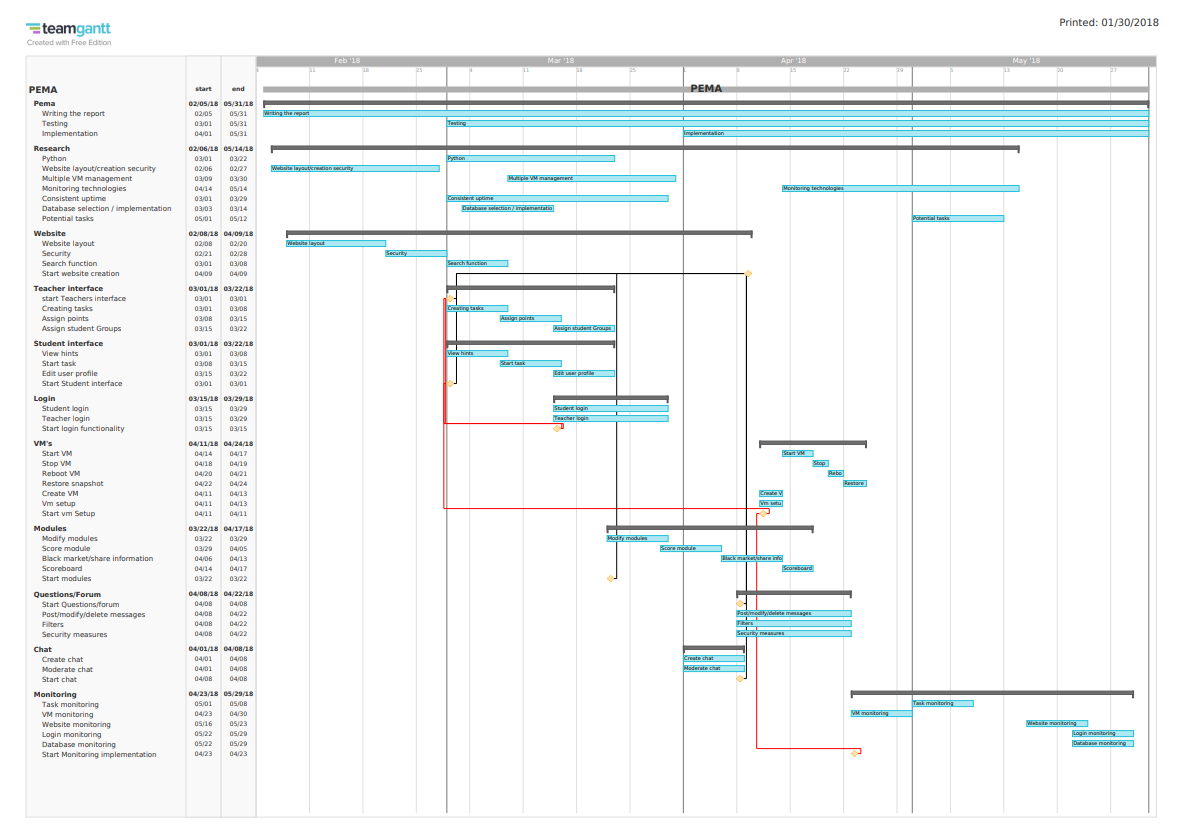
\includegraphics[scale=0.5]{Gantt.PNG}
\end{center}

\subsubsection{\textbf{Comments to the Gantt chart}}
Some of the Tasks are not mandatory to complete such as chat and monitoring which can be implemented at any time without a loss to the person using the website. 
Tho they are within the limits of what I want to achieve until the deadline and will attempt to do so, but if problems arrise they are the first ones to be cut from the finished project.






\end{document}
